\section{Quantum Optimal Control} \label{sec:QOC}

In the previous section we discussed the basics of adiabatic control and the toolbox of shortcuts to adiabaticity. That framework assumed that the initial and target states of a control problem are given in terms of eigenstates of our Hamiltonian for different values of the control parameter. In some scenarios, however, this might not be the case. In this section we introduce the tools of quantum optimal control, which will allow us to tackle arbitrary quantum control problems by systematically searching for the optimal form of the control fields that drive a quantum system to given target configuration. \steve{Typical optimal control implementations require repeated numerical evaluations of the full dynamics of a quantum system, and thus are often, in practice, restricted to small systems. Nevertheless, the success of optimal control techniques in solving control problems in few-body settings is a testament to its importance in the field. In the following we introduce and illustrate these tools by revisiting some of the models introduced in Sec. \ref{sec:STA} and analyzing them through the lens of optimal control. First, we will study optimal state control for a single qubit system obeying  the Landau-Zener Hamiltonian (c.f. Sec.~\ref{sec:LandauZener}), and then its extension to unitary gate preparation with a model of phase-only control. Finally, we will apply optimal control to the problem of generating entangled states in an extended version of the all-to-all Ising model introduced in Sec.~\ref{ex:LMGmodel}.}

% \steve{STEVE COMMENT: Add in a final sentence similar to the end of the STA section that explicitly says what examples will be considered.}\\
% \steve{FOR REFERENCE THIS IS FROM THE STA SECTION: We will explicitly consider the control of a simple two level system described by the Landau-Zener model in Sec.~\ref{sec:LandauZener}, which will serve as a paradigmatic example that will also be considered when discussing the other control techniques that are a focus of this tutorial, namely optimal control in Sec.~\ref{subsec:QOC_example_state} and reinforcement learning in Sec.~\ref{sec:RL_1q} and~\ref{sec:RL_2q}. We will also consider the application of these techniques to simple many-body settings embodied by three variations of the Ising model: (i) nearest neighbor, (ii) infinite range, and (iii) non-integrable.}

\subsection{Basic statement of an optimal control problem}
\label{subsec:QOC_intro}

In any quantum control problem, the goal is to maximize the success of a control protocol in driving a quantum system towards a predefined target configuration. For problems of state control, like the ones discussed in the previous section, this can be theoretically quantified by the quantum state fidelity, which measures how accurately the state at the final time $\ket{\psi(T)}$ approaches the target state $\ket{\psi_\ast}$ (typically, up to a global phase). This reads
\begin{equation}
    \mathcal{F}_S = \lvert \langle \psi_\ast |\psi(T)\rangle|^2,
\end{equation}
where $i\hbar \frac{d}{dt}\ket{\psi(t)}=H(t)\ket{\psi(t)}$. A more demanding control problem is that of unitary control, where we aim for the complete unitary evolution $U(T)$ to approach a target transformation $U_\ast$ (again up to a global phase). This will be the case, for instance, when the goal is to implement a quantum gate.  In such cases, the success of a protocol can be measured by 
\begin{equation}
    \mathcal{F}_U = \frac{1}{d^2}\left\lvert \Tr\left(U_\ast^\dagger U(T)\right)\right\rvert^2,
\end{equation}
 where now $i\hbar \frac{d}{dt}U(t)=H(t)U(t)$ and $d$ is the Hilbert space dimension. In this section, we introduce the tools of \textit{quantum optimal control} (QOC), which give a systematic approach to engineer $H(t)$ such that the target is approximately achieved, i.e., $\mathcal{F}\simeq 1$, where $\mathcal{F}$ symbolizes the state or unitary fidelities, depending on the problem at hand. Note that, depending on the specific control problem, alternative measures of protocol success can be defined. For instance, one could be interested in minimizing the energy of a system, or in achieving a specific expectation value of an observable. Here, for concreteness, we will focus on the use of the fidelity as such a measure.

We start by considering the system Hamiltonian $H(t)$ to be a function of a set of real \textit{control fields} $\bm{a}(t)=\{a_k(t)\}$, $j=1,\ldots,K$. For instance, we could consider the Hamiltonian to be written as
\begin{equation}
    H(t) = H_0 + H_C(t) = H_0 + \sum\limits_{k=1}^K a_k(t) H_{C,k},
    \label{eq:QOC_hami}
\end{equation}
which makes explicit the existence of a drift (or free) Hamiltonian $H_0$, which we cannot manipulate directly, and the control Hamiltonian $H_C(t)$, which depends on time through the control fields $\bm{a}(t)$ modulating the individual operators $H_{C,k}$. The properties of the drift and control Hamiltonians determine which states and transformations are in principle reachable to the system. Well-established methods to characterize this aspect exist \cite{dalessandro_book,poggi2019geometric}, and use tools rooted in Lie group theory to determine the degree of controllability of a given model.

Here we take a pragmatic approach, and establish a systematic way to find the control functions $\bm{a}(t)$ that minimize a \textit{cost functional}
\begin{equation}
    J[\bm{a}(t)] = 1-\mathcal{F}[\bm{a}(t)]
    \label{eq:QOC_functional}
\end{equation}
where $\mathcal{F}$ refers to either the state or unitary fidelity, and we have indicated the functional dependence of the fidelity explicitly. Note that here we follow the convention of defining a functional to be \textit{minimized}; one could similarly define a functional to be maximized instead. We will focus on solving this problem via numerical optimization, for which we introduce a parametrization of the control fields in terms of real numbers
\begin{equation}
    \bm{\alpha}=(\alpha_1,\alpha_2,\ldots,\alpha_M) \rightarrow \bm{a}(t),
    \label{eq:QOC_parametrization}
\end{equation}
which serve as a our control variables, and will allow us to treat the problem of minimizing Eq. (\ref{eq:QOC_functional}) with standard numerical optimization tools. Note that, while we do not treat them in this tutorial, there are approaches in optimal control theory which rely on functional optimization (see Krotov's method \cite{krotov1999,reich2012} and the \steve{Pontryagin} Maximum Principle~\cite{PRXQtutorial}). 

Generically, a numerical minimization routine involves initializing the controls with a guess $\bm{\alpha}_{0}$, and then iteratively updating it following a set of rules that depend on the optimization algorithm. These can be broadly classified as gradient-based and gradient-free depending on whether they compute derivatives of the cost function $J(\bm{\alpha})$ at various points to decide the most appropriate way to update the control field $\alpha(t)$ at each iteration. The choice of parametrization in Eq.~\eqref{eq:QOC_parametrization} is in principle arbitrary, but can be tailored to fit computational or experimental constraints. For instance, a Fourier parametrization would take the form
\begin{equation}
    \bm{\alpha} = (A_1,\ldots,A_{n_F},B_1,\ldots,B_{n_F})\rightarrow a(t) = \sum\limits_{m=1}^{n_F}\left[A_m \cos(\omega_m t) + B_m\sin(\omega_m t)\right], 
    \label{eq:QOC_fourier}
\end{equation}
where $n_F$ is the number of Fourier components and $\omega_m$ could correspond to the harmonics of some base frequency, or be chosen randomly (as in the chopped randomised basis, CRAB, algorithm \cite{doria2011_crab}). For concreteness, here we focus on parametrizing the field as a piecewise-constant function, 
\begin{equation}
\bm{\alpha} = (\alpha_1,\alpha_2,\ldots,\alpha_M)\rightarrow a(t) = \alpha_j\ \text{if}\ (j-1)\Delta t \leq t < j\Delta t,\ \text{where}\  j=1,\ldots,M.
\label{eq:QOC_pwc}
\end{equation}
where we have chosen a uniform time step $\Delta t$ for convenience. This choice is conceptually simple and allows us to analytically compute the gradient of the cost function of Eq. (\ref{eq:QOC_functional}) with respect to the control variables, which greatly improves the efficiency of the numerical search. We will work out this derivation explicitly in the next section.

\begin{table}[b]
\centering
\begin{tabular}{|p{12.5cm}|c|}
\hline
Object & Proposed Symbol \\
\hline\hline
Target state & $\ket{\psi_\ast}$ \\
\hline
Fidelity (state) & $\mathcal{F}_S$ \\
\hline
Target unitary & $\ket{U_\ast}$ \\
\hline
Fidelity (unitary) & $\mathcal{F}_U$ \\
\hline
Control field & $a(t)$ \\
\hline
Cost functional & $J[a(t)]$ \\
\hline
Control parameters & $\bm{\alpha}={\alpha_1,\ldots,\alpha_M}$  \\
\hline
Number of time steps & $M$\\
\hline 
Time step length & $\Delta t$ \\
\hline
Total evolution time & $T$ \\
\hline
Quantum speed limit time & $\tau_{\mathrm{QSL}}^\ast$ \\
\hline
\end{tabular}
\caption{Summary of notation for the most common quantities used in quantum optimal control.}
\label{table:QOCSymbols}
\end{table}
%--------------------------

\begin{figure}[t]
\centering
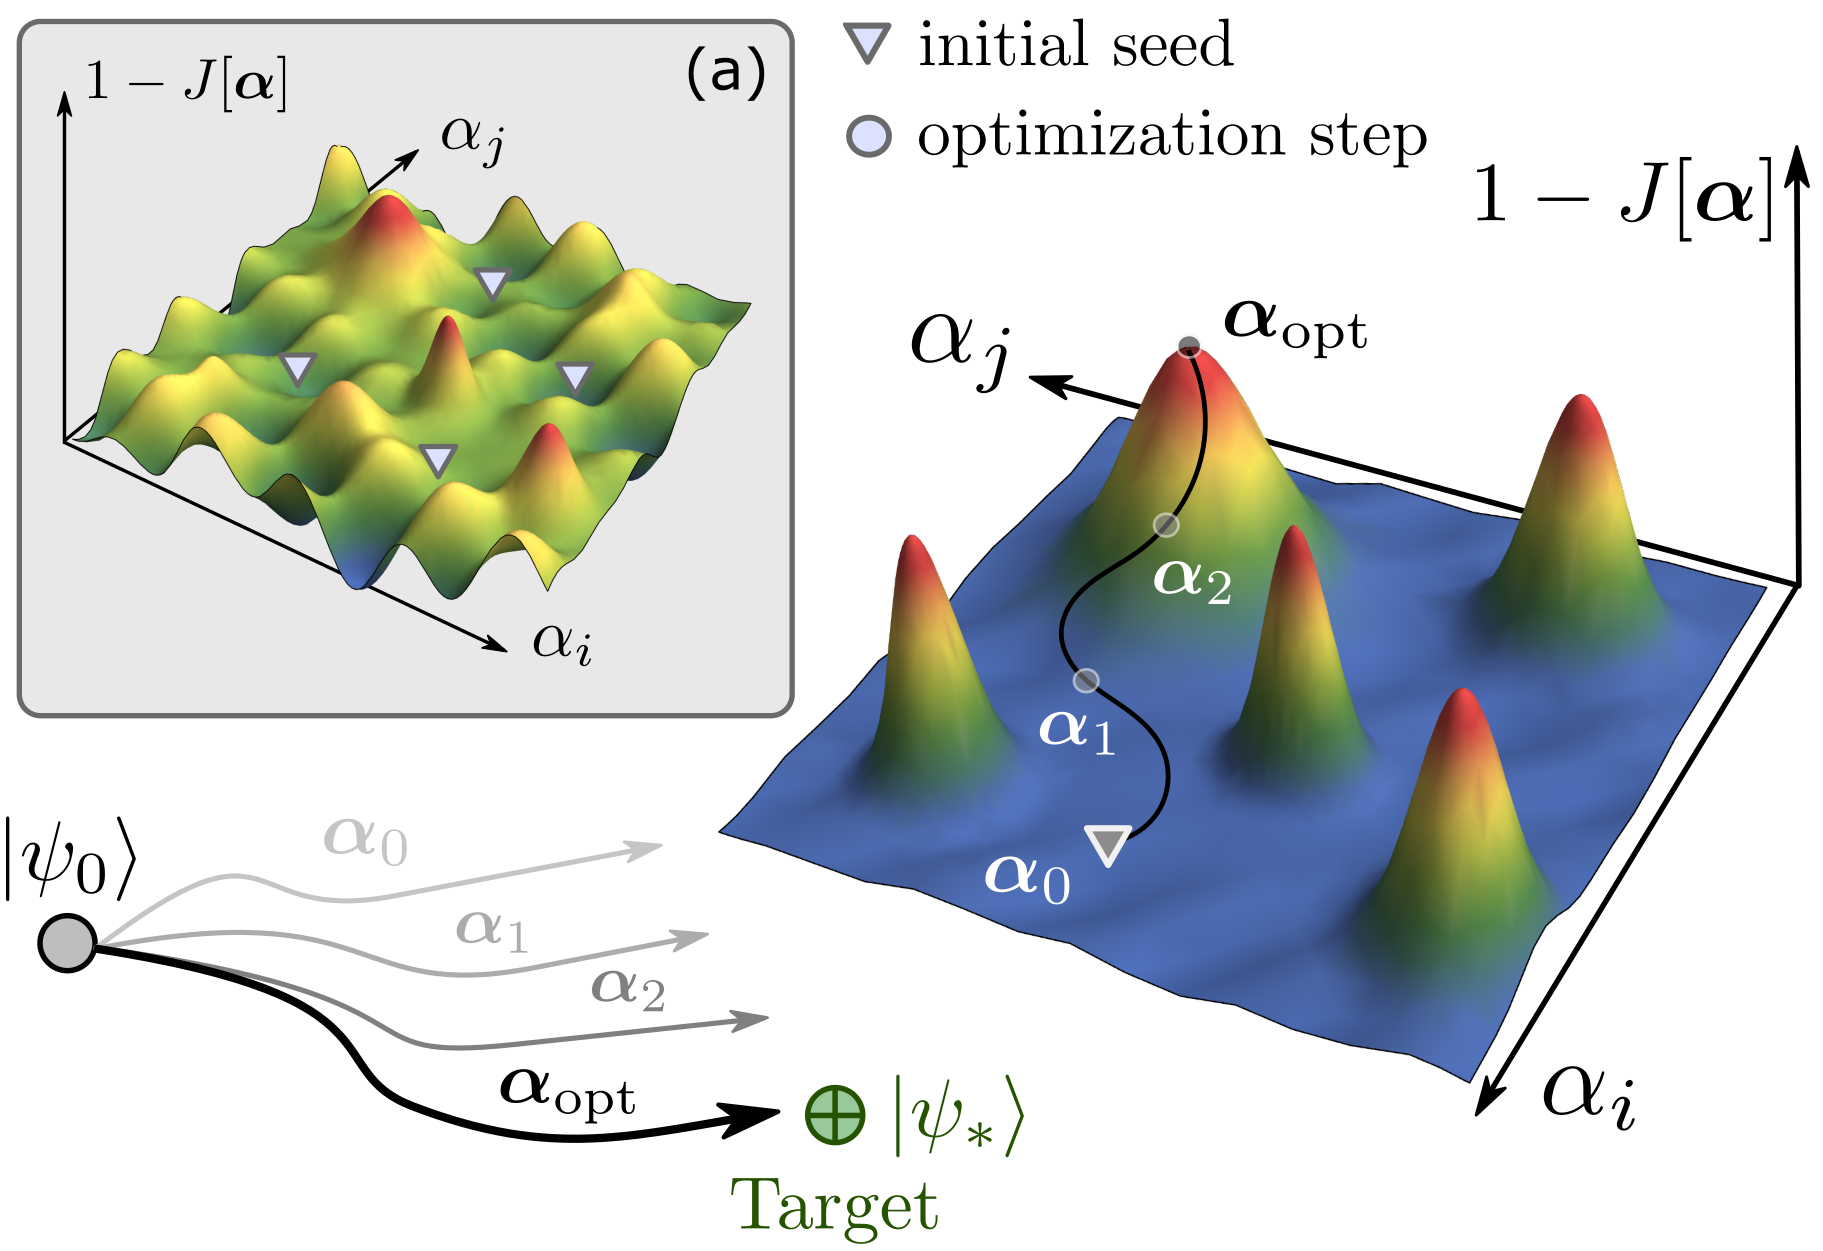
\includegraphics[width=0.55\columnwidth]{QOC_landscape.png}
\caption{Quantum control landscapes are determined by the dependence of the cost function $J(\bm{\alpha})$ on the control variables $\bm{\alpha}$. Main figure depicts how the optimal solutions, initial seeds, and optimization steps would appear in a two-dimensional landscape (note that real control problems typically have much more than $M=2$ dimensions). An optimization routine starts with an initial guess for the control variable $\bm{\alpha}_0$ which typically lands far from an extrema of the landscape, meaning that the evolution of the quantum state is far from the target configuration at the final time. The optimization consists in updating the control variables sequentially until an optimum is achieved $\bm{\alpha}_{\text{opt}}$. In the presence of constraints, quantum control problems can have rugged landscapes with suboptimal extrema, as depicted in subfigure (a). In such cases, using many different initial seeds helps explore various parameter regions of the landscape.}
\label{fig:QOC_landscapes}
\end{figure}


The definition of the control Hamiltonian, e.g. Eq. (\ref{eq:QOC_hami}), and parametrization, c.f. Eq. (\ref{eq:QOC_parametrization}), together with the choice of initial and target states ($\ket{\psi_0}$ and $\ket{\psi_\ast}$ for state control, $\mathds{1}$ and $U_\ast$ for unitary control), completely determine the cost function $J(\bm{\alpha})$, which can be seen as an optimization \textit{landscape}. Each point on the landscape corresponds to a different control field, with optimal protocols being global minima. The goal of any optimization algorithm is to traverse this landscape, starting from the initial guess $\bm{\alpha}_0$, to eventually reach the global extremum via a series of updates of the control parameters $\bm{\alpha}_0\rightarrow\bm{\alpha}_1\rightarrow \ldots \rightarrow \bm{\alpha}_{\text{opt}}$. Here, we assume that such updates are done via a local search (instead of a global one), where only properties about the current point and its surrounding region informs the update rule. This process is depicted in Fig. \ref{fig:QOC_landscapes}. The properties of the landscape determine the hardness of finding a solution to the control problem. In a generic optimization problem, the landscape is rugged and filled with suboptimal minima or traps, as can be seen in Fig.~\ref{fig:QOC_landscapes}(a), which often increases the computational expense of finding a near-optimal solution. In this scenario, it is typically convenient to balance the computational cost of the optimization between the exploration and the exploitation of the landscape. An optimization landscape can be explored by starting the search multiple times with different initial guesses (or ``seeds'') which aim to cover different regions of parameter space. Each run is then exploited by allowing the search a sufficient number of iterations to converge to a good solution.  For quantum control problems, remarkably, it has been shown that optimization landscapes tend to have benign features \cite{rabitz2004}; in particular, provided there are no constraints to the control \steve{problem} \cite{zhdanov2015}, quantum control landscapes can be shown to be generically devoid of traps \steve{in fully controllable systems} (see Fig. \ref{fig:QOC_landscapes}). \steve{In practice, however, constraints on control problems (which we discuss below) will typically affect the topology of control landscapes}. 
% \steve{REF COMMENT: There are a lot of caveats on this that are hard to satisfy especially in q. computing.} 
Interestingly, recent developments in quantum computing, particularly variational quantum algorithms, have revealed new properties of quantum control landscapes, like the phenomenon of barren plateaus, which we discuss briefly in Sec. \ref{outlook_sec_qc}.

Often, constraints need to be taken into account when solving practical quantum control problems, and thus understanding their effect on the optimization search is an important task. Constraints can be broadly divided into two categories: 
\begin{enumerate}
    \item Constraints which are \textbf{built into} the control model. For instance, a fixed set of control Hamiltonians in the expansion of Eq. (\ref{eq:QOC_hami}), a limited bandwidth set by the number of Fourier components in Eq. (\ref{eq:QOC_fourier}), or a limited evolution time $T = M\Delta t$ in Eq. (\ref{eq:QOC_pwc});
    \item Constraints which are imposed \textbf{a posteriori} to the problem as additional terms to the cost function. For instance, bounding the amplitude of driving field to limit its energetic cost \cite{reich2012} or demanding the control processes to be robust to certain external perturbations \cite{kosut2022,poggi2023_urc}.
\end{enumerate}

We highlight here the role of one of these constraints: limiting the total evolution time $T$. Quantum mechanics imposes fundamental limitations to the rate at which one state can evolve into a different state. These are formalized as quantum speed limits (QSLs)~\cite{Deffner2017}, which provide lower bounds on the total evolution time, c.f. $T\geq \tau_{\text{QSL}}$. For unitary dynamics, QSLs can be traced back to time-energy uncertainty relations, and take several forms \cite{taddei2013, pires2016, mondal2016,marvian2016}. In particular, we consider the bound derived from the work of Mandeltstam and Tamm \cite{mandelstam_45,bhattacharyya1983}:
\begin{equation}
    T \geq \frac{\hbar}{\overline{\Delta E}}\arccos\left(\lvert \langle \psi_\ast|\psi_0\rangle\rvert\right) \equiv \tau_{\text{QSL}},
    \label{eq:Tqsl}
\end{equation}
 where 
\begin{equation}
    \overline{\Delta E} = \frac{1}{T}\int\limits_0^T dt \Delta E(t)
\end{equation}
and $\Delta E(t)$ is the variance of the Hamiltonian $H(t)$,
\begin{equation}
    \Delta E(t)^2 = \bra{\psi(t)}H(t)^2\ket{\psi(t)}-\bra{\psi(t)}H(t)\ket{\psi(t)}^2.
\end{equation}
with $H(t)$ the total Hamiltonian, e.g. as defined in Eq.~\eqref{eq:QOC_hami}. The existence of QSLs fundamentally impacts quantum control problems as any optimization is destined to fail if one fixes the evolution time $T$ to be below $\tau_{\text{QSL}}$. Furthermore, it is usually desirable to derive control processes which are as fast as possible since long evolution times allow for more sources of errors and decoherence to affect the dynamics. While in some cases optimal control solutions exist exactly at the fundamental bound $T=\tau_\text{QSL}$ \cite{caneva2009}, typically constraints mean we can achieve  solutions only at longer times $\tau_\text{QSL}^\ast>\tau_\text{QSL}$ \cite{hegerfeldt2013,poggi2019geometric}. By definition, the time $\tau_\text{QSL}^\ast$ is the minimum possible evolution time for which a given optimal control problem has a solution (i.e., one that achieves a fidelity $\mathcal{F}=1$). In Sec. \ref{subsec:QOC_example_state} we will illustrate how to use optimal control methods to systematically search for the shortest evolution time $\tau_{\text{QSL}}^\ast$ for simple control problems, and explore how constraining the evolution time affects the optimization landscape. \steve{We point that out that geometric QSL bounds like Eq. (\ref{eq:Tqsl}), while universal, tend to become loose as the size of the system increases (see \cite{bukov2019geometric} for an exception) This is because the energy variance in the denominator is typically an extensive quantity.}

\subsection{Gradient-based optimal control using GRAPE} \label{subsec:QOC_grape}
In this section we discuss in more detail how to approach an optimal control problem numerically. We focus on the simplest case of having a single control field $a(t)$ parametrized with the piecewise constant ansatz of Eq. (\ref{eq:QOC_pwc}), leading to control variables grouped in a vector $\bm{\alpha}=\{\alpha_1,\alpha_2,\ldots,\alpha_M\}$. For a given choice of number of steps $M$ and total evolution time of $T$, the associated time step is $\Delta t=T/M$. This choice allows us to write the final-time evolution operator in closed form
\begin{equation}
    U(T) = U_M U_{M-1} \ldots U_2 U_1,\ \text{where}\  U_j = \exp\left(-iH_j\Delta t\right)\ \text{and}\ H_j =H(\alpha_j)
\end{equation}

To search for a choice of $\bm{\alpha}$ that minimizes the cost function $J(\bm{\alpha})$, one can resort to a variety of numerical optimization algorithms. Because we expect the cost function to have a smooth dependence on the control variables in general, it is convenient to use gradient-based methods, which use information about the derivatives $\partial J/\partial \alpha_k$ to inform the search at each step. Examples of these include gradient descent, Newton - Raphson and the Broyden-Fletcher-Goldfarb-Shannon (BFGS) algorithms. These are widely used optimization methods which are easily available in Python, Matlab, and other languages using standard packages (note that some quantum optimal control approaches also benefit from using gradient-free methods, like Nelder-Mead or Powell \cite{doria2011_crab,COLD_PRXQ}). For these methods, the computation of the gradient can be done numerically (e.g., via finite-difference approximations, which are typically carried out automatically by these optimization routines) or it can be provided explicitly such that it only has to be numerically evaluated. The piecewise-constant parametrization of the control field we are using here actually allows us to compute the gradient of $J(\bm{\alpha})$ analytically in a relatively straightforward way. The use of this parametrization together with the analytical form of the cost gradient in a quantum control problem constitutes the GRAPE (gradient-ascent pulse engineering) algorithm, first proposed by Khaneja \textit{et al.} \cite{khaneja2005}. 

To compute the gradient, we first note that for both state and unitary control problems the cost function can be written as $J(\bm{\alpha})=1-\mathcal{F}(\bm{\alpha})=1-|z(\bm{\alpha})|^2$ where
\begin{align}
\text{state control:} & \ z(\bm{\alpha})=\bra{\psi_\ast}U(T)\ket{\psi_0} \\
\text{unitary control:} & \ z(\bm{\alpha})=\frac{1}{d}\Tr\left(U_\ast^\dagger U(T)\right), 
\end{align}
and thus
\begin{equation}
    \frac{\partial J}{\partial \alpha_j} = \frac{\partial}{\partial \alpha_j}(z^\ast z) =  -2\Re{z^\ast \frac{\partial z}{\partial \alpha_j}}.
    \label{eq:QOC_gradZ}
\end{equation}

As the control dependence is entirely contained within $U(T)$, to obtain $\frac{\partial z}{\partial \alpha_j}$ we require to calculate
\begin{equation}
      \frac{\partial U(T)}{\partial \alpha_j} =U_M U_{M-1}\ldots \frac{\partial U_j}{\partial \alpha_j} U_{j-1}\ldots U_1
    \label{eq:QOC_gradient0}
\end{equation}
and thus we need to compute $\frac{\partial U_j}{\partial \alpha_j}$. Here, one should proceed with care because $U_j=\exp(-i H_j \Delta t)$ does not necessarily commute with $\partial H_j/\partial \alpha_j$. In general, we have

\begin{align}
    \frac{\partial U_j}{\partial \alpha_j} & = \frac{\partial}{\partial \alpha_j}\sum\limits_{k=0}^\infty \frac{(-i)^k}{k!}\Delta t^k H_j^k \\
    & = \sum\limits_{k=0}^\infty \frac{(-i)^k}{k!}\Delta t^k \sum\limits_{i=1}^k H_j^{i-1} \frac{\partial H_j}{\partial \alpha_j} H_j^{k-i}
    % & = \sum\limits_{k=0}^\infty \frac{(-i)^k}{k!}\Delta t^k \sum\limits_{i=1}^k H_j^{i-1} H_C H_j^{k-i}
    \label{eq:QOC_derUj_aj}
\end{align}

In the limit where the time step $\Delta t$ is small, and thus the piecewise constant field resembles a continuous function, the expression in Eq. (\ref{eq:QOC_derUj_aj}) can be simplified, see for instance Ref. \cite{khaneja2005,ansel2024_arxiv}. For that limit to be relevant, however, we need to deal with a large number $M$ of control variables, which can be undesirable. Here we focus on obtaining an exact closed form for $\partial U_j/\partial \alpha_j$, valid for arbitrary time step sizes $\Delta t$ \cite{machnes2011,motzoi2011}. For this, we introduce the spectral decomposition of $H_j = \sum_{l=1}^d e_l \ketbra{l}{l}$ (note that both the eigenvalues and eigenvectors will be different for each $j$, i.e. for each time step). Inserting this into Eq. (\ref{eq:QOC_derUj_aj}), we obtain

\begin{align}
    \frac{\partial U_j}{\partial \alpha_j} & = \sum\limits_{k=0}^\infty \frac{(-i)^k}{k!}\Delta t^k \sum\limits_{i=1}^k \sum\limits_{l,m} e_l^{i-1}e_m^{k-i} \ketbra{l}{m} \bra{l}\frac{\partial H_j}{\partial \alpha_j}\ket{m} \nonumber \\
    & = \sum\limits_{l,m} \ketbra{l}{m} \bra{l}\frac{\partial H_j}{\partial \alpha_j}\ket{m} \sum\limits_{k=0}^\infty \frac{(-i)^k}{k!}\Delta t^k \sum\limits_{i=1}^k e_m^{k-1} \left(e_l/e_m\right)^{i-1}.
    \label{eq:QOC_gradient1}
\end{align}

The infinite series appearing in the above expression can be evaluated exactly. For the case $e_l = e_m$, we obtain

\begin{equation}
    \sum\limits_{k=0}^\infty \frac{(-i)^k}{k!}\Delta t^k k e_m^{k-1} = -i\Delta t \sum\limits_{k=0}^\infty \frac{(-i)^{k-1}}{(k-1)!}\Delta t^{k-1} e_m^{k-1}=-i\Delta t \exp{-i e_m \Delta t}.
    \label{eq:QOC_gradient2}
\end{equation}

If $e_l\neq e_m$, we can proceed as follows
\begin{align}
    \sum\limits_{k=0}^\infty \frac{(-i)^k}{k!}\Delta t^k e_m^{k-1}\sum\limits_{i=1}^k \left(e_l/e_m\right)^{i-1} & = \sum\limits_{k=0}^\infty \frac{(-i)^k}{k!}\Delta t^k \frac{e_m^k}{e_m}\sum\limits_{n=0}^{k-1} \left(e_l/e_m\right)^{n} \nonumber \\
    & = \sum\limits_{k=0}^\infty \frac{(-i)^k}{k!}\Delta t^k \frac{e_k^k - e_m^k}{e_l-e_m} \nonumber \\
    & = \frac{1}{e_l-e_m}\left(e^{-i e_l \Delta t}-e^{-i e_m \Delta t}\right).
    % -i\Delta t \exp\left(\frac{e_l+e_m}{2}\right)\text{sinc}\left(\frac{e_l+e_m}{2}\right),
    \label{eq:QOC_gradient3}
\end{align}

Combining expressions (\ref{eq:QOC_gradient1}), (\ref{eq:QOC_gradient2}) and (\ref{eq:QOC_gradient3}) yields an analytical expression for all the matrix elements of $\partial U_j/\partial \alpha_j$. Notice that this requires us to diagonalize the operator $H_j$ for each $\alpha_j$, which will need to be done numerically in most cases. For a single qubit, the eigenvectors and eigenvalues of $H_j$ have a analytic form for an arbitrary $\alpha_j$. Here we do not use this form to illustrate the more general procedure, which applies to more complex systems. Once the factor from Eq. (\ref{eq:QOC_gradient1}) is computed, the gradient can be constructed from Eq. (\ref{eq:QOC_gradient0}),

\begin{align}
    \text{state control:} & \     \frac{\partial z}{\partial \alpha_j} = \bra{\psi_\ast}U_{j+1,M}\frac{\partial U_j}
    {\partial \alpha_j}U_{1,j-1}\ket{\psi_0}\\
    \text{unitary control:} & \ \frac{\partial z}{\partial \alpha_j} = \frac{1}{d}\Tr\left(U_\ast^\dagger U_{j+1,M}\frac{\partial U_j}
    {\partial \alpha_j}U_{1,j-1}\right)
\end{align}
where we introduced the notation $U_{k,l}=U_l U_{l-1}\ldots U_{k+1}U_k$. Note that in the case of state control, the cost function gradient at step $j$ depends on the initial state $\ket{\psi_0}$ forward-evolved until time-step $j-1$, and on the target state $\ket{\psi_\ast}$ backwards-evolved until time-step $j+1$.\\

We can now construct a basic optimal control routine by following these steps:

\begin{enumerate}
    \item Set the final evolution time $T$ and the number of timesteps $M$ (which defines the number of control variables). This suffices to define a discretized time variable $t\rightarrow \{t_k = k\Delta t\}$, with $k=0,1,\ldots,M$, and $M\Delta t=T$.
    \item Choose an initial guess or ansatz $\bm{\alpha}_0$ for the control variable. 
    \item Implement a numerical minimization routine. Typical inputs for such routine are
    \begin{itemize}
        \item The cost function $J(\bm{\alpha})$.
        \item The particular minimization method to be used (BFGS, gradient descent, ...)
        \item The associated gradient function $g(\bm{\alpha})=\frac{\partial}{\partial \bm{\alpha}}J(\bm{\alpha})$, Eq. (\ref{eq:QOC_gradZ}).
        \item The initial guess $\bm{\alpha}_0$, defined in step 2.
        \item Bounds on the control variables such that the search is restricted to $\alpha_{min}\leq \alpha_j \leq \alpha_{max}$ (optional)
        \item Numerical tolerances or thresholds on the cost and/or the gradient, which determine at what level of precision the search is allowed to stop.
    \end{itemize}
\end{enumerate}


In the remainder of this section, we consider two examples in which we illustrate this procedure for both state and unitary control in a two-level system.

% \pablo{We attach to this Tutorial  example scripts that implement all these steps in Python, using optimization routines from the Scipy package}. 

\subsection{Examples}
\subsubsection{Example: optimal control in the Landau-Zener model}
\label{subsec:QOC_example_state}
We begin by considering control of the Landau-Zener Hamiltonian, already introduced in Sec. \ref{sec:LandauZener}, which has the form 
\begin{equation}
    H(t) = H_0 + \nu(t) H_C = \Delta \sigma^x + \nu(t) \sigma^z.
    \label{eq:QOC_hami_LZ}
\end{equation}
We also recall here the form of the ground state of $H(t)$ as a function of instantaneous value of $\nu(t)$:
\begin{equation}
    \ket{\phi_g(\nu)} \equiv \cos\left(\frac{\theta}{2}\right) \ket{0}+\sin\left(\frac{\theta}{2}\right) \ket{1},\ \text{with}\ \tan\theta = \frac{\Delta}{\nu}.
\end{equation}
For this model we are interested in the problem of driving the system from the initial state 
\begin{equation}
    \ket{\psi_0}=\ket{\phi_g(-\nu_0)}
\end{equation}
to the target state
\begin{equation}
    \ket{\psi_\ast}=\ket{\phi_g(+\nu_0)}
\end{equation}
for some $\nu_0>0$. Note that, as $\nu_0\rightarrow \infty$, we have $\theta\rightarrow 0 $ and the desired evolution is the one that connects $\ket{\psi_0}=\ket{0}$ to $\ket{\psi_\ast}=\ket{1}$. We consider the field $\nu(t)$ to be piecewise-constant with $M=10$ steps and denote its values $\{\alpha_1,\ldots,\alpha_M\}$ to make notation consistent with the previous section. Note that this example obeys the decomposition of Eq. (\ref{eq:QOC_hami}). Even in this very simple case, one finds that $H_j = H_0+\alpha_j H_C$ and $\partial H_j/\partial \alpha_j=H_C=\sigma^z$ do not commute, which motivates the need for the calculation of the gradient shown in Sec. \ref{subsec:QOC_grape}.\\

To test the optimization procedure of steps 1-3 above, we start by fixing $T=\pi/\Delta$, and using a limited-memory variant of the BFGS method (L-BFGS-B) as our optimization routine. We also restrict the search to $|\alpha_j|\leq c = 2\Delta$ to avoid control fields with large amplitudes. With these specifications, we run the optimal control routine for two choices of the parameter $\nu_0$ determining the initial and target states ($\nu_0=1$ and $\nu_0=5$), and two choices of initial ansatz; one where the $\alpha_j$'s are sampled from a uniform distribution between $[-1,1]$, and another where we choose $\alpha_j=0$ for all $j=1,\ldots,M$. Results are shown in Fig.~\ref{fig:QOC1}, where we display the initial guess for the control field (gray dashed lines) and the optimal field obtained with the optimization routine (colored full lines). In all cases we observe that the cost function is initially of order $J(\bm{\alpha}_0) \in (0.5 , 1)$, and that the optimization is able to achieve $J(\bm{\alpha}_{\text{opt}})\in \left( 10^{-16},10^{-13}\right)$ in any standard run. Comparison of Figs.~\ref{fig:QOC1} (a)-(b) and (c)-(d) reveals that for a given control problem (i.e., for a fixed $\nu_0$), different initial guesses perform similarly. The comparison also illustrates two generic facts of quantum optimal control. \steve{When the system is controllable and given enough control resources,} control problems typically have multiple possible solutions which are (roughly) equally good. Even for fixed, finite values of $T$ and $M$ (which effectively impose constraints on the control problem) these multitude of solutions can be accessed by exploration of the control landscape with different initial guesses $\bm{\alpha_0}$ (see illustration in Fig. \ref{fig:QOC_landscapes}). \steve{In addition}, the optimal fields often inherit properties of the initial guesses. This is because in presence of multiple minima,  a local optimization routine like the one considered here will lead to a solution close to the initial point. In our example, we see that the optimal fields obtained following the random ansatz look random themselves, while the optimal fields obtained from the constant initial guess are reveal to be structured and symmetric. For simple systems like the one studied here, these features might be easily traced back to symmetries of the model \cite{larocca2018} but, in more complex cases, the structure of the optimal field can be useful to identify nontrivial properties of the system \cite{rabitz2006_topology,poggi2015,bukov2018_symmetry}. \\

\begin{figure}[t]
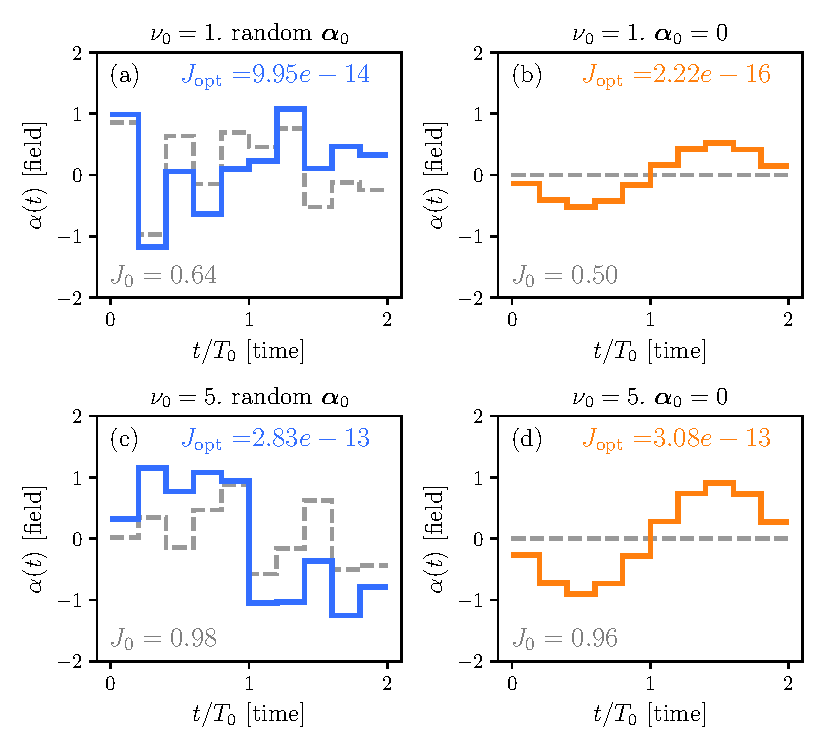
\includegraphics[width=0.55\columnwidth]{QOC-Fig1-A.pdf}
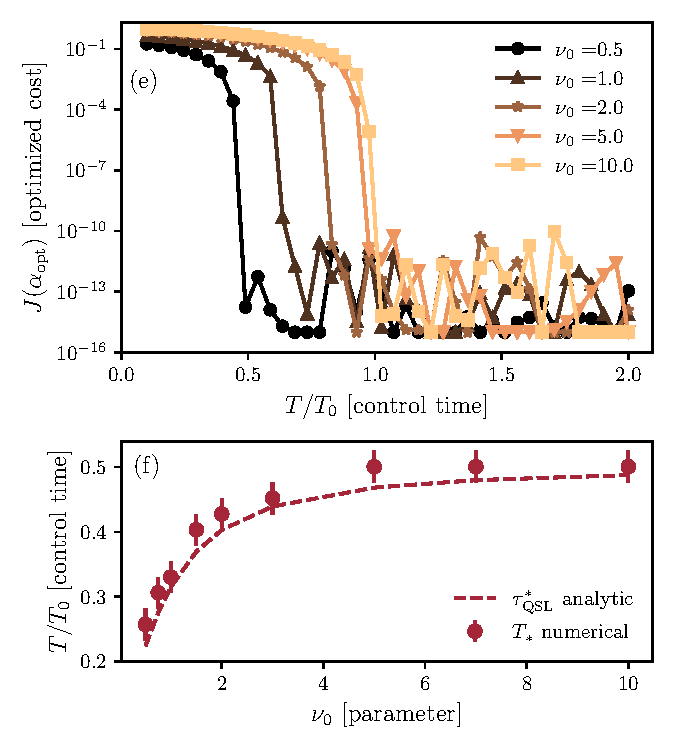
\includegraphics[width=0.43\columnwidth]{QOC-Fig1-B.pdf}
\caption{Quantum optimal state control for the Landau-Zener model. (a)-(d) Show various control fields related to realizing a state transfer process between ground states of the Landau-Zener Hamiltonian, c.f. Eq. (\ref{eq:QOC_hami_LZ}). Shown are the initial guesses (gray dashed lines) and optimized fields (thick colored lines) for four different cases. (a) Initial state given by $\nu_0=1$, and initial guess for control field $\bm{\alpha}_0$ chosen randomly. (b) $\nu_0=1$ and $\bm{\alpha}_0=0$. (c) $\nu_0=5$ and $\bm{\alpha_0}$ random. (d) $\nu_0=5$ and $\bm{\alpha}_0=0$. In all cases the initial $J_0\equiv J({\bm{\alpha}_0})$ and optimized $J_{\mathrm{opt}}\equiv J(\bm{\alpha}_{\mathrm{opt}})$ values of the cost function are displayed. Parameters used $M=10$, $T=2T_0$ where $T_0=\pi/(2\Delta)$. (e) Optimized cost functions achieved by the optimization as a function of total evolution time $T$, for various choices of the parameter $\nu_0$ determining the initial and final state. (f) Minimum control time for the Landau-Zener Hamiltonian, as a function of $\nu_0$. Circles indicate the numerical estimates obtained from the data shown in (e). Full line corresponds to the analytical solution derived in Ref. \cite{hegerfeldt2013}.}
\label{fig:QOC1}
\end{figure}

% \steve{REF COMMENT: This is only possible in small systems}
{\it Identifying quantum speed limits using optimal control.---} Following on from previous discussions on quantum speed limits, it is natural to ask what is the minimum evolution time $\tau_{\text{QSL}}^\ast$ required to achieve a good solution for this control problem. To explore this question, we set out to solve the optimization problem for different values of the total evolution time $\{T_1,T_2,\ldots,T_R\}$, arranged in increasing order. In principle, each choice of $T$ leads to an independent optimization procedure, given by the steps 1-3 above. Here we describe a slightly more elaborate approach, which has been routinely used in previous studies \cite{caneva2009,murphy2010,goerz2011,poggi2015_qsl,goerz2017, ref2, ref3, ref4}. We start by solving the optimal control problem for the largest value of evolution time $T_R$ with a given choice of initial ansatz $\bm{\alpha}_0^{(R)}$ (say, a uniformly random one). If $T_R>\tau_{\text{QSL}}^\ast$, then we expect to be able to obtain an optimal field $\bm{\alpha}_{\text{opt}}^{(R)}$ yielding a very small cost function. We then move on to solve the optimization for $T_{R-1}$, but now we choose as an initial guess the optimal field from the previous run, i.e.
\begin{equation}
    \text{initial guess for $T=T_{j-1}$}\rightarrow \bm{\alpha}_0^{(j-1)} =  \bm{\alpha_{\text{opt}}^{(j)}}\leftarrow \text{optimal field from $T=T_j$}.
\end{equation}
When repeating this procedure for every choice of $T$ in our list, we are ``helping'' each new optimization by seeding a field which we expect to lead to a small cost (as long as $T_j-T_{j-1}$ is sufficiently small). In Fig.~\ref{fig:QOC1}(e)  we plot the optimized cost as a function of the evolution time $T$ for this procedure, for various choices of $\nu_0$ (i.e. for various choices of initial and target states). Analyzing the curves starting from the right (large values of $T$), in all cases we observe nearly optimal fidelities, corresponding to costs of orders between $10^{-12}$ and $10^{-15}$. As the allowed evolution time decreases, the optimization is able to find good solutions up until a critical time, after which the optimized cost grows rapidly and takes values $\sim 10^{-1}$. This critical time $T_*$ divides the controllable regime where $T>T_*$ and the uncontrollable regime where $T<T_*$. Because $T_*$ depends on details of the optimization procedure (for instance, on the number of time steps $M$), it can only provide  an upper bound to the true minimum control time $\tau_{\text{QSL}}^\ast$. Nevertheless, in many situations of interest, we can take $T_*$ as a good approximation of $\tau_{\text{QSL}}^\ast$. For the problem treated here, the actual optimal time is known analytically \cite{hegerfeldt2013,poggi2013}. In Fig. \ref{fig:QOC1}(f) we compare the numerically obtained $T_*$ and the analytical $\tau_{\text{QSL}}^\ast$ as a function of $\nu_0$. The results indicate that the numerical optimal control procedure is able to obtain good estimates of the fundamental optimal control time for this problem. In particular, we see how as $\nu_0\rightarrow \infty$ and thus $\ket{\psi_0}\rightarrow \ket{0}$ and $\ket{\psi_\ast}\rightarrow\ket{1}$, the control time reaches $\tau_{\mathrm{QSL}}^\ast=\frac{\pi}{2\Delta}$. This is the time required by $H=\Delta \sigma_x$ to rotate $\ket{0}$ to $\ket{1}$. 

\subsubsection{Example: optimal control of a single-qubit gate}
\label{subsec:QOC_example_gate}
\begin{figure}[t]
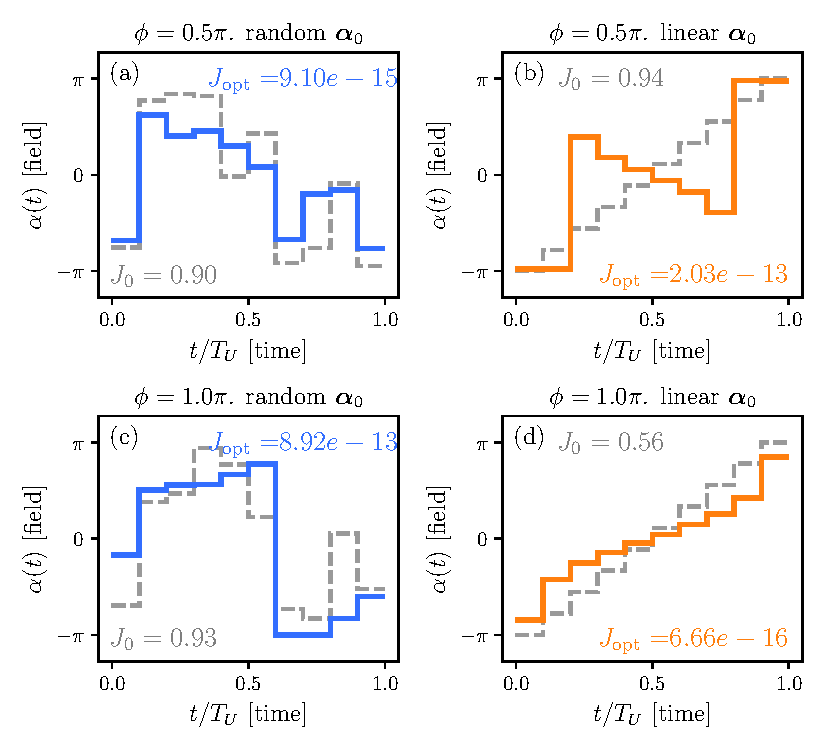
\includegraphics[width=0.55\columnwidth]{QOC-Fig2-A.pdf}
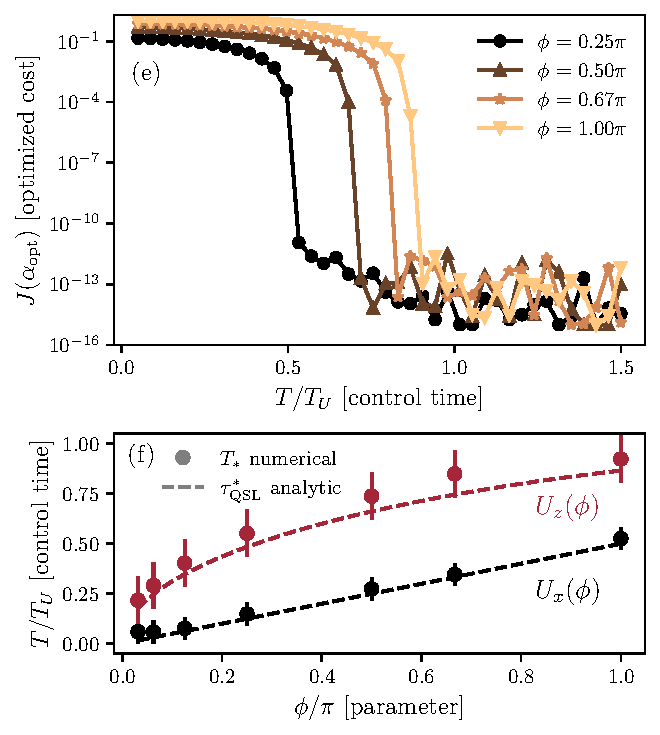
\includegraphics[width=0.43\columnwidth]{QOC-Fig2-B.pdf}
\caption{Quantum optimal control for a single-qubit gate. (a)-(d) Show control fields related to implementing the target gates $U_z(\phi)$ in Eq. (\ref{eq:QOC_gate_target_z}) using the control Hamiltonian in Eq. (\ref{eq:QOC_gate_hami}). We display
initial guesses (gray dashed lines) and optimized fields (thick colored lines) for four different cases. (a) Target gate given by $\phi=\pi/2$, and initial guess for control field $\bm{\alpha}_0$ chosen randomly. (b) $\phi=\pi/2$ and $\bm{\alpha}_0$ linear. (c) $\phi=\pi/2$ and $\bm{\alpha}_0$ random. (d) $\phi=\pi$ and $\bm{\alpha}_0$ linear. In all cases the initial $J_0\equiv J({\bm{\alpha}_0})$ and optimized $J_{\mathrm{opt}}\equiv J(\bm{\alpha}_{\mathrm{opt}})$ values of the cost function are displayed. Parameters used $M=10$, $T=T_U$, where $T_U=2\pi/\Omega$. (e) Analysis of optimal cost functions achieved by the optimization as a function of total evolution time $T$, for various choices of the target $U_z(\phi)$.
(f) Minimum control time as a function of $\phi$ for the two families of target gates $U_x(\phi)$ and $U_z(\phi)$. Circles indicate the numerical estimates obtained from the optimal control procedure. Dashed lines correspond to analytical solutions. For $U_x$, $\tau_{\mathrm{QSL}}^\ast/T_U=\phi/(2\pi)$. For $U_z$ the optimal evolution time has been derived in Ref. \cite{boozer2012}.}
\label{fig:QOC2}
\end{figure}



Here we consider a different model of a two-level system where we aim at generating unitary transformations, or gates, using optimal control. To this effect, we will study the Hamiltonian
\begin{equation}
    H(t) = \frac{\Omega}{2}\left( \cos(\alpha(t)) \sigma_x + \sin(\alpha(t)) \sigma_y\right).
    \label{eq:QOC_gate_hami}
\end{equation}
This model corresponds to a single spin-$1/2$ particle being driven by a field with constant amplitude $\Omega$ (i.e. Rabi frequency) but variable direction in the $x\!-\!y$ plane, determined by $\alpha(t)$. When compared to the Landau-Zener Hamiltonian, c.f. Eq. (\ref{eq:QOC_hami_LZ}), this model has two important features. First, the energy of the system is bounded by $\Omega/2$ irrespective of the control field. Thus, increasing the amplitude or frequency of the field will not necessarily make the system evolve faster in time. Second, it does not follow the decomposition of Eq.~(\ref{eq:QOC_hami}). In particular, one finds that $\partial H_j/\partial \alpha_j$ is now a function of $\alpha_j$ due to the nonlinear dependence on the control field. Nonetheless, this case is naturally contemplated in the general calculation of the gradient of Sec. \ref{subsec:QOC_grape}. 

In a unitary control problem, we need to define the target transformation. We consider two families of target gates,
\begin{align}
    U_x(\phi) &= \exp\left(-i \sigma_x \phi/2\right), \label{eq:QOC_gate_target_x}\\
    U_z(\phi) &= \exp\left(-i \sigma_z \phi/2\right). \label{eq:QOC_gate_target_z}
\end{align}
Note that for the targets $U_x(\phi)$, the problem has a straightforward solution, obtained by setting $\alpha(t)=0$ and evolving the system for a time $T=\phi/\Omega$. On the other hand, for the case $U_z(\phi)$ the control field needs to play a nontrivial role to generate the desired gate. 

We analyze this problem numerically by choosing the field $\alpha(t)$ to be piecewise-constant with $M=10$, as in the previous example. We start considering an evolution time of $T=2\pi/\Omega$ and two instances of the target gates $U_z(\phi)$ with $\phi=\pi/2$ and $\phi = \pi$. To illustrate the results of the search, we again consider two different types of initial guess: control parameters randomly sampled from a uniform distribution in $[-\pi,\pi]$, or increasing linearly in time from $-\pi$ at $t=0$ to $\pi$ at $t=T$. Results are shown in Fig. \ref{fig:QOC2}. Similarly to the results displayed in the previous section, we observe how the optimization routine is able to decrease the value of the cost by over 10 orders of magnitude and achieve very high fidelities. We also observe how different initializations of the search lead to different optimal fields, which inherit properties of the initial seed.\\

Finally, we can use our optimization procedure to explore the quantum speed limit to achieve the indicated target gates. We do this in exactly the same way as described for the state control problem in the previous section. In Fig.~\ref{fig:QOC2}(e) we show the optimized cost values as a function of evolution time $T$ for the gates $U_z(\phi)$ and various choices of $\phi$. We observe a clear separation between the controllable regime for $T>\tau_{\text{QSL}}^\ast$ where very low cost values are achievable, and the uncontrollable regime where $T<\tau_{\text{QSL}}^\ast$ and the optimal cost is highly constrained. The critical evolution time $T_*$ increases with $\phi$, which is intuitive as gates with larger $\phi$ are further away from the identity, i.e. the initial state for unitary control. A deeper analysis of this feature is presented in Fig.~\ref{fig:QOC2}(f), revealing a  square-root-like growth of $T_*$ with $\phi$. This is consistent with the actual minimum evolution time $\tau_{\text{QSL}}^{*(z)}$ which for this problem has been analytically obtained in Ref.~\cite{boozer2012}. For completeness, we include results corresponding to the family of gates $U_x(\phi)$ for which, as mentioned before, optimization was not really necessary. Nonetheless, we verify with numerical optimization that it is not possible to break the minimum evolution time given by $\tau_{\text{QSL}}^{*(x)} = \phi/\Omega$, which scales as $\phi$ instead of $\sqrt{\phi}$. Similarly to what happens with state control problems and the quantum speed limit, lower bounds to the minimum control times can be obtained via geometric arguments~\cite{poggi2019geometric}.

\subsubsection{Example: generation of many-body entanglement}



The examples shown in the Secs. \ref{subsec:QOC_example_state} and \ref{subsec:QOC_example_gate} showcase the application of QOC to the simplest model of a two-level system or qubit.  One obvious extension of these cases is the generation of two-qubit gates, which has been thoroughly studied for various platforms, including superconducting qubits, trapped ions, and neutral atoms. Nevertheless, the formalism described in Sec. \ref{subsec:QOC_grape} is general and can be directly applied to more complex scenarios.\\

Here we consider the problem of many-body state preparation, which is closely related to the control tasks treated in Sec. \ref{sec:RL_theory} with the STA formalism. While the direct application of QOC to many-body systems is naturally limited by the computational complexity of numerically simulating these systems, we will show that even for modest system sizes QOC can provide interesting insights into the resources needed to perform control on a high-dimensional Hilbert space. This, in turn, will allow us to address a key point raised in Sec. \ref{sec:Introduction}: the use of quantum control tools to bridge the gap between implementability and scalability of quantum operations. \\

We consider a model of $N$ qubits undergoing global control and all-to-all interactions according to the Hamiltonian

\begin{equation}
    H(t) = \frac{\Omega_x(t)}{2}\sum\limits_{i=1}^N \sigma_i^x + \frac{\Omega_y(t)}{2}\sum\limits_{i=1}^N \sigma_i^y + \frac{\beta}{4N}\sum\limits_{i,j=1}^N \sigma_i^z \sigma_j^z
    \label{eq:QOC_hami_many_body}
\end{equation}

Note that, as opposed to the single-qubit example, here the model has a drift term which is time-independent (thus, not directly controllable), which corresponds to the interaction between the qubits. The relevant time-scale of the problem is set by $T_\beta=2\pi/\beta$. We have also chosen to normalize the interaction term to ensure that the Hamiltonian remains extensive as $N$ increases. 

We consider the following control task. Starting from the state

\begin{equation}    \ket{\psi_0}=\ket{00\ldots 0},
\end{equation}
we want our system to reach an entangled state $\ket{D_k^{(N)}}$ characterized by the symmetric superposition of all possible $k$ bit-flips. For instance, if $N=4$ some of the target states we are interested in are 
\begin{align}
    \ket{D_1^{(N=4)}} &= \frac{1}{2}\left(\ket{1000}+\ket{0100}+\ket{0010}+\ket{0001}\right)\\
    \ket{D_2^{(N=4)}} &= \frac{1}{\sqrt{6}}\left(\ket{1100}+\ket{1010}+\ket{1001}+\ket{0110}+\ket{0101}+\ket{0011}\right)
\end{align}

These types of states display multipartite entanglement, and are regarded as a resource in quantum sensing \cite{toth2012} and cavity quantum optics \cite{pezze2018}, among others. \\

To tackle this problem, we first note that the Hamiltonian in Eq. (\ref{eq:QOC_hami_many_body}) is invariant under any permutation of the qubits. This allow us to write this operator elegantly in terms of collective spin operators
\begin{equation}
    J_\alpha = \frac{1}{2} \sum\limits_{i=1}^N \sigma_i^\alpha,
\end{equation}
leading to

\begin{equation}
    H(t) = \Omega_x(t) J_x + \Omega_y(t) J_y + \frac{\beta}{N} J_z^2.
\label{eq:QOC_hami_spinJ}
\end{equation}

In this form, it also becomes clear that at all times $[H(t),\mathbf{J}^2]=0$, where $\mathbf{J}^2=J_x^2+J_y^2+J_z^2$ is the total spin of the system. In addition, the set of initial and target states all correspond to joint eigenstates of $J_z$ and $\mathbf{J}^2$ (note that $\ket{\psi_0}=\ket{D_0^{(N)}}$). These are also called Dicke states, which obey \cite{dicke1954}
\begin{align}
    J_z \ket{D_k^{(N)}} &= \left(\frac{N}{2}-k\right)\ket{D_k^{(N)}} \\
    \mathbf{J}^2 \ket{D_k^{(N)}} &= \frac{N}{2}\left(\frac{N}{2}+1\right)\ket{D_k^{(N)}}.
\end{align}

Thus, our control problem takes place in a reduced subspace spanned by these states, which has a dimension $N+1$, as the value of excitations $k$ goes from 0 to $N$. This reduced subspace is actually exactly equivalent to the Hilbert space of a single spin-$J$ particle with $J=N/2$. In fact, the Hamiltonian in Eq. (\ref{eq:QOC_hami_spinJ}) accurately models the dynamics of electronic states in individual atoms, where the $J_z^2$ now corresponds to a non-linear light-shift induced by non-resonant optical driving \cite{deutsch2010}. These systems are now routinely being considered as qudits for quantum computing platforms, and the results shown here directly carry over to that application as well \cite{omanakuttan2021} (see also Sec. \ref{outlook_sec_qc} for further information).\\

With this model we can explore how control resources change as the complexity of the control task increases, both in terms of increasing the number of target excitations $k$ and the number of total particles $N$. To do this, we run the QOC procedure outlined in Sec. \ref{subsec:QOC_grape} to this problem for $N=6,8,10$ particles, and in each case to reach a target state with $k=1,2,..,N/2$ excitations. We note that the case $k>N/2$ turns out to be equivalent to the cases considered here, up to global rotations. \\

Similar to the analysis shown in, e.g., Fig. \ref{fig:QOC1} (e), we run the optimization for various choices of the total evolution time, in order to identify an approximate quantum speed limit required to produce these various transformations. Results are shown in Fig. \ref{fig:QOC3}. For each value of $N$ considered, we find that the time required for the control to find high-fidelity solutions does not depend significantly on the number of excitations $k$ in the target state. This indicates that even when states with higher $k$ require more bit-flips, the optimal solution is able to efficiently navigate Hilbert space and takes a shortcut to generate the target state directly. In turn, by comparing the curves for different values of $N$, we do observe that the total amount of time increases with system size in a seemingly linear fashion. This is expected given the linear increase of accessible Hilbert space. We note that this is also a consequence of the choice of normalization in Eq. (\ref{eq:QOC_hami_many_body}).

\begin{figure}[t]
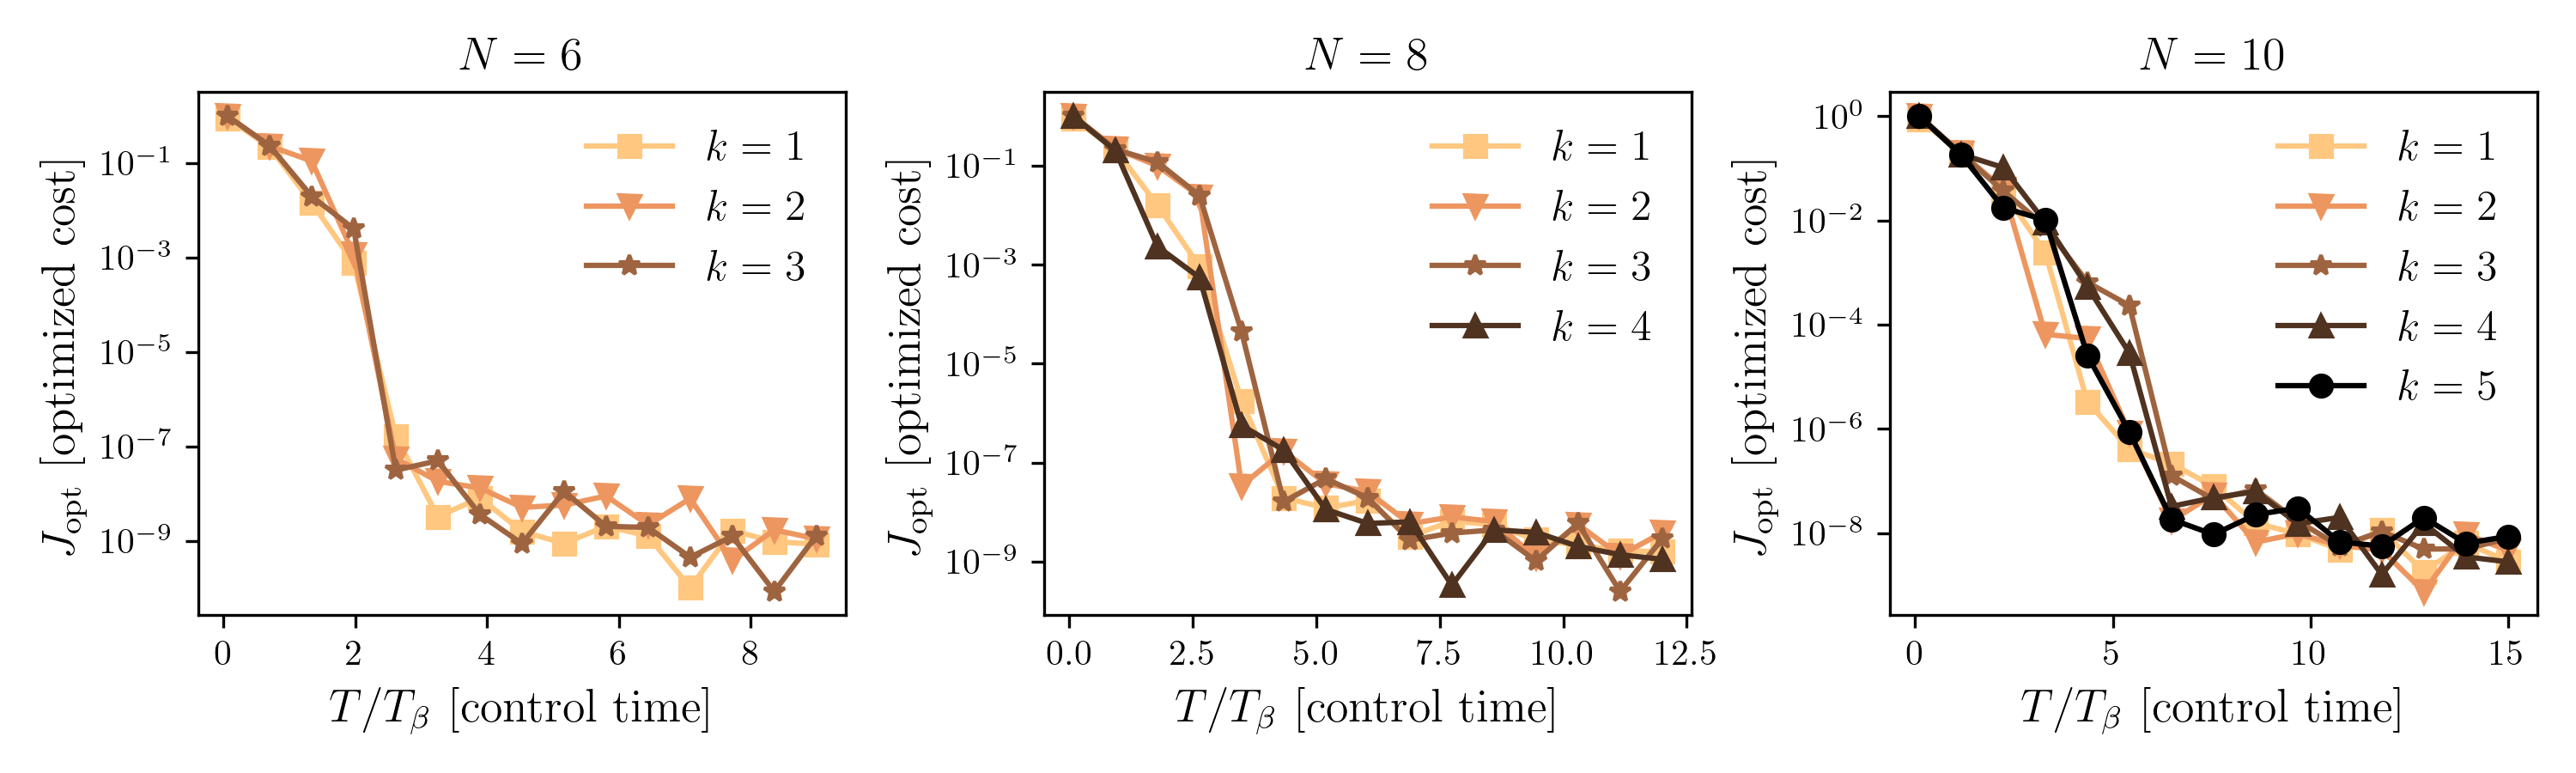
\includegraphics[width=\columnwidth]{QOC-Fig3.png}
\caption{Quantum optimal control for many-body entangled state generation. Panels show the optimized cost obtained from QOC on the protocol described in the main text, as a function of the allotted control time $T$. In all cases, both fields $\Omega_x(t)$ and $\Omega_y(t)$ are discretized with $M=15$ steps and constrained to maximum amplitude of $\Omega_{\mathrm{max}}=3\beta$.} 
\label{fig:QOC3}
\end{figure}


\subsection{Experimental implementations of quantum optimal control}
Quantum optimal control tools have been successfully applied to various experimental platforms involving manipulation of quantum systems. Interestingly, the flexibility of QOC has led each community to adapt these tools to tackle and mitigate errors and limitations which are native to each implementation. Following the discussion in Sec.~\ref{subsec:QOC_intro}, this translates into imposing different constraints to the base QOC problem. Examples of this include leaking reduction in superconducting qubits~\cite{motzoi2009} and inhomogeneous broadening mitigation in atomic and nuclear magnetic resonance (NMR) systems~\cite{ruths2012}.

Here we name some examples of successful implementations of QOC in different platforms, in a manifestly non-exhaustive way; the reader is referred to Reviews such as Refs.~\cite{Glaser2015,Koch2022} for further examples. In atomic systems, optimal control has been used to coherently control large manifolds of electronic states in individual neutral atoms. This includes both Zeeman \cite{smith2013,anderson2015,lysne2020} and Stark states \cite{larrouy2020}. In these cases both radiofrequency and microwave fields are modulated in time to achieve the desired control. Demonstrated tasks include the generation of circular Rydberg and nonclassical superposition states, as well the implementation of arbitrary unitary operations within the corresponding electronic state manifold.

Likewise, QOC has become a standard tool to design entangling gates between neutral atoms for quantum computing. In this case, time-modulation of laser intensity and detuning can be optimized to produce operations which are highly robust to imperfections like light shift broadening or spontaneous decay. Recent demonstrations which leverage QOC tools include Refs.~\cite{omran2019,evered2023,cao2024}. A similar approach has been applied to trapped-ion quantum processors, with entangling gates enabled by optimal design of frequency comb structure~\cite{choi2014}. These systems have also benefited from QOC in the task of transporting individual ions along a trap~\cite{sterk2022}.

Superconducting circuits have also successfully implemented optimal control tools for various tasks. In these systems, control is exerted by microwave signals; recently demonstrated tasks include the implementation of a universal gate set on a logical cat qubit~\cite{heeres2017} and high-fidelity qudit gates~\cite{seifert2023}. Since superconducting qubits are two-levels embedded in a larger Hilbert space, it is crucial to minimize population leaking outside of the relevant computational subspace. The DRAG (derivative removal by adiabatic gate) method is a QOC approach that has been proposed to address this issue~\cite{motzoi2009}, and which has been experimentally demonstrated in Ref.~\cite{werninghaus2021}. Following its demonstrated success and flexibility, quantum optimal control is now becoming an industrial standard for quantum computing, with many quantum hardware and software providers utilizing quantum control tools in various layers of the computing stack for tasks like circuit compilation, gate synthesis, state preparation and readout, and error mitigation.

Finally, we briefly mention that quantum optimal control tools have a long history beyond the quantum information processing platforms mentioned here. In particular, optimization is a standard tool in composite pulse design in NMR experiments~\cite{bonnard2012}. Also, the control of chemical reactions using shaped laser pulses was one of the first applications of quantum optimal control theory, see for instance Ref.~\cite{tannor1985}.

%\clearpage

% \subsection{Worked Example on Geometric Gates--Likely to be commented out.}
% \textbf{Note that several things in this example have overlap with 
% general stuff above, so need to edit this out later on!}

% \paragraph*{Intro.}
% The following example features the 
% example of a so-called \textit{geometric gate}, which is a useful 
% concept in many different quantum technology platforms that are 
% based on qubits, hence it has great generality. Here we will 
% focus on a single qubit, but note that the principle of geometric
% gates can be extended to two- or multi-qubit gates as well. 
% The exposition here is mainly based on the discussion in 
% \cite{daems2013} and \cite{xu2020}.

% \paragraph*{Setup.}
% Denoting the qubit ground and excited states as $|0\rangle$ and $|1\rangle$, 
% respectively, we must find the wave function $|\psi(t)\rangle$ at 
% all subsequent times by solving
% \begin{align}
% i\frac{\partial}{\partial t}|\psi(t)\rangle=H_d(t)|\psi(t)\rangle,
% \end{align}
% where $H_d(t)$ a the time-dependent driving Hamiltonian to control 
% the qubit system. 

% We can infer a lot of information about the state of the system 
% simply by the fact that whatever $H_d(t)$ may be, the state will 
% have to be parametrized by some curve in the Hilbert space of a 
% qubit, i.e. on the Bloch sphere. From elementary expositions, we 
% know that a state at some time $t_0$ can be parametrized by two angle on the Bloch sphere, 
% $\alpha$ and $\beta$ according to 
% \begin{align}
% |\psi(t_0)\rangle=\cos\frac{\alpha}{2} e^{-i\beta/2}|0\rangle+\sin\frac{\alpha}{2} e^{i\beta/2}|1\rangle,
% \end{align}
% up to a global phase factor.
% For a time-dependent Hamiltonian, we can use a similar parametrization 
% of the state, but now with time-dependent angles, $\alpha(t)$ and $\beta(t)$, 
% according to 
% \begin{align}
% |\psi(t)\rangle=e^{-i f(t)/2}\left[\cos\frac{\alpha(t)}{2} e^{-i\beta(t)/2}|0\rangle
% +\sin\frac{\alpha(t)}{2} e^{i\beta/(t)2}|1\rangle\right].
% \end{align}
% Here $f(t)$ is a function that describes an overall phase \cite{daems2013}, 
% whose significance we will soon see.
% Likewise, since the Schr{\"o}dinger equation generates unitary time-evolution, 
% we can infer that there is another states orthogonal to $|\psi(t)\rangle$ at 
% all times, that we parametrize as 
% \begin{align}
% |\phi(t)\rangle=e^{i f(t)/2}\left[-\sin\frac{\alpha(t)}{2} e^{-i\beta(t)/2}|0\rangle
% +\cos\frac{\alpha(t)}{2} e^{i\beta/(t)2}|1\rangle\right],
% \end{align}
% and one easily checks that $\langle\phi(t)|\psi(t)\rangle=0$ for any $\tau$. This will 
% be handy to describe the general gate operation.

% To implement a geomtric gate, we must modulate the parameters in $H_d(t)$
% to that we make a closer curve within the Hilbert space of the qubit. 
% Assuming that the evolution takes place within a time $0\leq t\leq \tau$, 
% we require $\alpha(0)=\alpha(\tau)$ and $\beta(0)=\beta(\tau)$. Hence, 
% the state is the same except for a global phase factor 
% \begin{align}
% \gamma=\frac{f(0)-f(\tau)}{2}=\gamma_D+\gamma_G
% \end{align}
% that has a dynamical and a geometric contribution. The
% dynamical contribution is 
% \begin{align}
% \gamma_D=-\in\tau_{0}^{\tau} \langle \psi(t)|H_d(t)|\psi(t)\rangle,
% \end{align}
% while the geometric phase is given by the formula
% \begin{align}
% \gamma_G=i\in\tau_{0}^{\tau} \langle \tilde\psi(t)|\frac{\partial}{\partial t}|\tilde\psi(t)\rangle,
% \end{align}
% where for convenience, we have introduced $|\tilde\psi(t)\rangle=e^{if(t)/2}|\psi(t)\rangle$.
% Note the latter does not depend on the Hamiltonian, but rather on the path and 
% the change in the state in Hilbert space during the evolution. This is 
% the origin of the name, geometric phase. 

% To achieve a geometric gate, we need to eliminate the effect of the 
% dynamical phase, and hence we assume that we make a global phase change 
% at $t=\tau$ such that we can assume $\gamma_D=0$. Note that we did not 
% discuss any conditions of adiabatic evolution, and the discussion is 
% in principle general thus far. Hence, we can use non-adiabatic 
% changes in the driving Hamiltonian, but of course the concrete setting
% and platform will set the limits on how this may impact the dynamics. 
% For example, typical qubits consist of an effective two-level subspace
% of a quantum system with other states in the spectrum, and we still need
% to observe population into those states, and counteract those effects by 
% carefully tailored driving protocols as discuss earlier. 

% \paragraph*{A single-qubit geometric gate.}
% Assuming $\gamma_D=0$, we have $\gamma=\gamma_G$ at time $t=\tau$. 
% We can now write down the total effect of the time-evolution on 
% the system by observing that $|\psi(t)\rangle$ and $|\phi(t)\rangle$
% will accumulate phases $\gamma$ and $-\gamma$, respectively. Hence, we
% can write the unitary operator responsible for the dynamics from 
% $t=0$ to $t=\tau$ as 
% \begin{align}
% U(\tau)=e^{i\gamma}|\psi(t)\rangle\langle\psi(t)|+
% e^{-i\gamma}|\phi(t)\rangle\langle\phi(t)|.
% \end{align}
% Since we are assuming that 
% $\alpha(0)=\alpha(\tau)$ and $\beta(0)=\beta(\tau)$, we may insert the 
% two states and obtain the matrix form
% \begin{align}
% U(\tau)=
% \left[
% \begin{matrix}
% \cos\gamma+i\cos\alpha\sin\gamma & i\sin\gamma\sin\alpha\, e^{-i\beta}\\
% i\sin\gamma\sin\alpha\, e^{i\beta} & \cos\gamma-i\cos\alpha\sin\gamma
% \end{matrix}
% \right],
% \end{align}
% where $\alpha=\alpha(0)$ and $\beta=\beta(0)$ are the starting angles 
% of the time-evolution. This can also be written in terms of the 
% Pauli matrices in operator form
% \begin{align}
% U(\tau)=\exp\left(i\gamma \vec{n}\cdot \vec{\sigma}\right),
% \end{align}
% where $\vec{n}=(\sin\alpha\cos\beta,\sin\alpha\sin\beta,\cos\alpha)$ 
% is a unit vector and $\vec{\sigma}$ is the 
% vector of Pauli matrices. According to the usual conventions of 
% operators acting on a qubit, this operation is a rotation around 
% the spin-space axis $\vec{n}$ by an angle $-2\gamma$. 
% Hence, we have effectively applied a geometric 
% single-qubit gate, and can pick among different options by 
% using the boundary conditions given by $\alpha$ and $\beta$.

% \paragraph*{An example.}
% We now consider an example of a driving Hamiltonian
% \begin{align}
% H_d(t)=
% \frac{1}{2}\left[
% \begin{matrix}
% 0 & \Omega(t) \\
% \Omega(t) & 0 
% \end{matrix}
% \right],
% \end{align}
% which corresponds to a laser field or microwave fields driving with 
% time-dependent Rabi frequency $\Omega(t)$, and we have assume that
% the driving Hamiltonian is real for simplicity. 

% TO do: WRITE EQUATIONS, DISCUSS X GATE, INTRODUCE OPTIMAL CONTROL.
